\chapter{Loi exacte pour le modèle \acs{CGL}}
\renewcommand\partie{\Partie\ Chapitre \thechapter}
\label{ch-21}

\bigskip
\minitoc  

Dans le vent solaire, utiliser un modèle \ac{MHD} compressible avec pression isotrope peut s'avérer ardu à justifier en présence d'un champ magnétique et d'un faible nombre de collisions. Il faut prendre en compte, a minima, une pression gyrotrope par exemple en utilisant le modèle dit \ac{CGL}. C'est le but de ce chapitre : décrire la cascade turbulente d'énergie totale à travers une loi exacte associée au modèle \ac{CGL}. Encore une fois, on ne réduira le champ d'application qu'après avoir obtenu une loi plus générale, valable pour tout tenseur de pression. Les nouveaux résultats exposés ici ont fait l'objet principal de l'article [\cite{simon_exact_2022}].

\section{D'un tenseur de pression dans le modèle fluide au modèle \acs{CGL} }
\label{sec-211}

Dans le cadre général défini à partir de l'équation de Vlasov et menant au modèle \ac{MHD}, la pression et le flux de chaleur sont définis comme des tenseurs d'ordre 2 et 3 respectivement. La pression, $\overline{\boldsymbol{P}} $, est un tenseur symétrique obtenu en effectuant le produit de deux vecteurs vitesse tandis que le flux de chaleur s'obtient à partir du produit de trois vecteurs vitesse. 

 Dans la Partie \ref{part_1}, la pression était supposée isotrope, c'est à dire $\overline{\boldsymbol{P}} = p \overline{\boldsymbol{I}}$ avec $\overline{\boldsymbol{I}}$ le tenseur identité. Dans le modèle \ac{CGL}, elle est définie comme gyrotrope par rapport à la direction du champ magnétique, notée $\boldsymbol{b}$. On considère donc deux pressions, une dite parallèle $p_{\parallel}$ et une perpendiculaire $p_{\perp}$ et dans un repère cartésien orienté tel que $\boldsymbol{b}$ coïncide avec la direction $\boldsymbol{e_z}$, le tenseur s'écrit : 
\begin{equation*}
 \overline{\boldsymbol{P}} = \left( \begin{array}{ccc}
                                    p_{\perp} & 0 & 0 \\
                                    0 & p_{\perp} & 0 \\
                                    0 & 0 & p_{\parallel} 
                                    \end{array} \right).   
\end{equation*}
Plus généralement, on peut l'écrire : $ \overline{\boldsymbol{P}} = p_{\perp} \overline{\boldsymbol{I}} + \left(p_{\parallel} - p_{\perp}\right) \boldsymbol{b}\boldsymbol{b} $. La partie isotrope de la pression est obtenue en faisant le produit dual "$:$" entre $\overline{\boldsymbol{P}}$ et  $\overline{\boldsymbol{I}}$, ce qui revient à considérer la trace de $\overline{\boldsymbol{P}}$. Ainsi : $p = \frac{1}{3} \overline{\boldsymbol{P}} : \overline{\boldsymbol{I}} = \frac{1}{3} \left(2 p_{\perp} + p_{\parallel} \right) $. Cela permet de réécrire le tenseur de pression en séparant la partie isotrope de la composante dite anisotrope : $\overline{\boldsymbol{P}} = p \overline{\boldsymbol{I}} + \left(p_{\parallel} - p_{\perp}\right)\left(\boldsymbol{b}\boldsymbol{b} - \frac{1}{3} \overline{\boldsymbol{I}} \right)$, on notera la composante anisotrope $\overline{\boldsymbol{\Pi}}$. Dans le cas général non-gyrotrope, d'autres composantes apparaissent. On n'abordera pas leur détail et on les résumera simplement par la notation $\overline{\boldsymbol{\Pi}}_{ng}$. D'après \cite{cassak_pressure-strain_2022}, $\overline{\boldsymbol{\Pi}} = \left(p_{\parallel} - p_{\perp}\right)\left(\boldsymbol{b}\boldsymbol{b} - \frac{1}{3} \overline{\boldsymbol{I}} \right) + \overline{\boldsymbol{\Pi}}_{ng}$ contribue à la déformation incompressible du fluide par compression/expansion et cisaillement à travers le terme $\overline{\boldsymbol{P}} : \nabla \boldsymbol{v}$ tandis que $p$ résulte en sa dilatation, compressible. En mécanique des fluides, ces termes de pression anisotrope sont souvent une réécriture des termes de dissipation visqueuse d'où leur interprétation dissipative. 

On rappelle le modèle non fermé dépendant des moments $\rho, \boldsymbol{v}, \overline{\boldsymbol{P}}$ et $\overline{\overline{\boldsymbol{q}}}$ et de la loi d'Ohm \acs{MHD} exprimée à travers l'équation d'induction \eqref{eq:model_cpg_b} : 
\begin{eqnarray}
\label{eq:model_cpg_r} \partial_t \rho + \nabla \cdot \left(\rho \boldsymbol{v}\right) &=& 0,\\
\label{eq:model_cpg_v} \partial_t \left(\rho \boldsymbol{v}\right) + \nabla \cdot \left(\rho \boldsymbol{v}\boldsymbol{v} - \rho \boldsymbol{v_A}\boldsymbol{v_A}\right) +  \nabla \overline{\boldsymbol{P_*}}  &=& 0 , \\
\label{eq:model_cpg_P} \partial_t \overline{\boldsymbol{P}} + \nabla \cdot \left( \boldsymbol{v} \overline{\boldsymbol{P}} \right) +  \left(\overline{\boldsymbol{P}} \cdot \nabla \boldsymbol{v}\right)^S + \omega_{ce} \frac{|\boldsymbol{v_A}|}{v_{A0}} \left(\boldsymbol{b}\times \overline{\boldsymbol{\Pi}}_{ng}\right)^S  & =& - \nabla \cdot \overline{\overline{\boldsymbol{q}}} ,\\
\label{eq:model_cpg_b} \partial_t \boldsymbol{v_A} -  \nabla \cdot \left(\boldsymbol{v_A}\boldsymbol{v} - \boldsymbol{v}\boldsymbol{v_A}\right) +  \boldsymbol{v} \nabla \cdot \boldsymbol{v_A} -  \frac{\boldsymbol{v_A}}{2}  \nabla \cdot \boldsymbol{v} &=& 0 ,
\end{eqnarray}
sachant que $\boldsymbol{b}\times \overline{\boldsymbol{I}} = 0$ et $\boldsymbol{b}\times \boldsymbol{b}\boldsymbol{b} = 0$, et en notant $\overline{\boldsymbol{P_*}} = \overline{\boldsymbol{P}} + p_m \overline{\boldsymbol{I}}$, le tenseur de pression totale. Aucune hypothèse sur la forme des tenseurs de pression et flux de chaleur n'est faite dans ce modèle. 

Ce modèle peut nous servir à obtenir une loi exacte générale sur l'énergie totale applicable sous l'hypothèse d'une cascade isentrope, quelles que soient les formes de la pression et du flux de chaleur. En effet, comme dans le cas avec pression isotrope, l'équation \eqref{eq:model_cpg_P} ne servira pas dans la dérivation de la loi exacte. On utilisera seulement l'équation d'énergie interne que l'on peut obtenir à partir de l'équation sur la composante isotrope du tenseur de pression : 
\begin{equation}
\label{eq:model_cpg_p}     \partial_t p + \nabla \cdot \left(p \boldsymbol{v} \right) + \frac{2}{3} \overline{\boldsymbol{P}} : \nabla \boldsymbol{v}   = - \frac{1}{3} \nabla \cdot \left(\overline{\overline{\boldsymbol{q}}} : \overline{\boldsymbol{I}}\right)
\end{equation}
puisque $\overline{\boldsymbol{\Pi}}_{ng}$ étant symétrique $\left(\boldsymbol{b}\times \overline{\boldsymbol{\Pi}}_{ng}\right):\overline{\boldsymbol{I}} = 0$.
L'énergie interne sera définie par $\rho u = \frac{1}{2} \overline{\boldsymbol{P}} : \overline{\boldsymbol{I}} = \frac{3}{2} p = \frac{1}{2} \left(2 p_{\perp} + p_{\parallel} \right) $, la dernière formulation étant associée au cas particulier gyrotrope [\cite{hazeltine_local_2013}].
On retrouve donc l'équation \eqref{eq:synth_cpi_u} écrite pour un tenseur de pression quelconque : 
\begin{equation}
\label{eq:model_cpg_u}     \partial_t \left(\rho u\right) + \nabla \cdot \left(\rho u \boldsymbol{v} \right) +  \overline{\boldsymbol{P}} : \nabla \boldsymbol{v}   = - \frac{1}{2} \nabla \cdot \left(\overline{\overline{\boldsymbol{q}}} : \overline{\boldsymbol{I}}\right) .
\end{equation}
Cette équation est assez générale et peut être obtenue indépendamment de l'expression de $u$ en fonction de $p$ et de l'équation \eqref{eq:model_cpg_P}, avec un bilan énergétique, comme celui que l'on a effectué dans le Chapitre \ref{ch-12} [\cite{eckart_thermodynamics_1940,hazeltine_local_2013}]. On peut y faire apparaître l'isentropie à travers l'hypothèse : $ \nabla \cdot \left(\overline{\overline{\boldsymbol{q}}} : \overline{\boldsymbol{I}}\right) = 0$.  

La fermeture \ac{CGL} consiste à annuler la divergence du flux de chaleur $\nabla \cdot \overline{\overline{\boldsymbol{q}}}$ dans l'équation \eqref{eq:model_cpg_P} et à considérer un tenseur de pression de forme gyrotrope. L'équation tensorielle de pression prend alors la forme de deux équations (voir [\cite{hunana_introductory_2019}] pour les détails de dérivations) : 
\begin{eqnarray}
\label{eq:model_cpg_ppar}     \partial_t p_{\parallel} + \nabla \cdot \left(p_{\parallel} \boldsymbol{v} \right) + 2 p_{\parallel} \boldsymbol{b}\boldsymbol{b} : \nabla \boldsymbol{v}   &=& 0 \\
\label{eq:model_cpg_pperp}     \partial_t p_{\perp} + \nabla \cdot \left(p_{\perp} \boldsymbol{v} \right) + p_{\perp} \nabla \cdot \boldsymbol{v}- p_{\perp} \boldsymbol{b}\boldsymbol{b} : \nabla \boldsymbol{v}   &=& 0 
\end{eqnarray}
En les sommant, on retrouve l'équation d'énergie interne \eqref{eq:model_cpg_u} avec l'hypothèse d'isentropie. Pour simplifier les calculs dans cette Partie \ref{part_2}, nous supposerons, dans le cas général, $\nabla \cdot \overline{\overline{\boldsymbol{q}}} = 0$ (équation \eqref{eq:model_cpg_P}). Cette hypothèse est, comme on vient de le voir, cohérente avec l'hypothèse d'isentropie de la cascade turbulente et avec le modèle \ac{CGL} qui nous intéresse. Elle pourra être facilement relaxée, si besoin est, en prenant en compte, dans la loi exacte, la correction \eqref{eq:turb_ref_q} qui a été dérivée dans la section \ref{sec-133}.

En manipulant les équations de pression du modèle \ac{CGL}, \eqref{eq:model_cpg_ppar} et \eqref{eq:model_cpg_pperp}, avec l'équation d'induction \eqref{eq:model_cpg_b}, on obtient les formes conservatives : 
\begin{equation}
\label{eq:model_cpg_biadiab}    d_t \left(\frac{p_{\parallel}\boldsymbol{v_A}^2}{\rho^2}\right) = 0\qquad d_t \left(\frac{p_{\perp}}{\rho^{3/2} |\boldsymbol{v_A}|}\right)=0
\end{equation}
De ce lien, entre $p_{\parallel,\perp}$ et des puissances de $\rho$, provient la deuxième appellation du modèle, <<bi-adiabatique>>, et les formes explicites des pressions : $p_{\parallel} \propto \frac{\rho^2}{\boldsymbol{v_A}^2}$ et $p_{\perp}\propto \rho^{3/2} |\boldsymbol{v_A}|$. 

\section{Instabilités linéaires et potentiel impact sur la turbulence du vent solaire}
\label{sec-212}

Les anisotropies de pression peuvent rendre le plasma instable. On utilise la théorie linéaire pour approcher ce problème comme on a approché celui des ondes d'Alfvén et magnétosonores dans les modèles \ac{MHD} (voir Chapitres \ref{ch-11} et \ref{ch-12}). Le pendant non linéaire de ces instabilités est en effet difficile à établir. 

La linéarisation du modèle \ac{CGL} (voir méthode dans la section-synthèse du Chapitre \ref{ch-11} et pour plus de détails, le chapitre 3 de [\cite{hunana_introductory_2019}]) nous donne l'équation de dispersion $\overline{\boldsymbol{M}}\cdot \boldsymbol{v_1} = 0$ avec : 
\begin{equation}
 \overline{\boldsymbol{M}} =    \begin{pmatrix}
\label{eq:lin_cpg_eqdis}  M_{xx}   & 0 & -  \frac{\beta_{\parallel 0}}{2} a_{p0}  \frac{k_{\perp}}{k_{\parallel}} \\
    0 &  M_{yy} & 0 \\
      - \frac{\beta_{\parallel 0}}{2} a_{p0} \frac{k_{\perp}}{k_{\parallel}} & 0 &\frac{\omega^2}{ v^2_{A0}k^2_{\parallel}} -  \frac{3}{2} \beta_{\parallel 0}  
    \end{pmatrix} 
\end{equation}
et 
\begin{eqnarray*}
    M_{xx} &=& \frac{\omega^2}{v^2_{A0}k^2_{\parallel}} -  \left(\beta_{\parallel 0} a_{p0}+1\right)  \frac{k^2_{\perp}}{k^2_{\parallel}} +   \left(\frac{\beta_{\parallel 0}}{2} \left(1-a_{p0}\right)-1\right) , \\
    M_{yy}& =& \frac{\omega^2}{v^2_{A0}k^2_{\parallel}} +   \left(\frac{\beta_{\parallel 0}}{2} \left(1-a_{p0}\right)-1\right) .
\end{eqnarray*}
$a_{p0} = \frac{p_{\perp 0}}{p_{\parallel 0}}$ est le taux d'anisotropie et $\beta_{\parallel 0} = \frac{2 p_{\parallel 0}}{\rho_0 v^2_{A0}}$ est le paramètre $\beta$ linéaire du plasma calculé avec la pression parallèle. La relation de dispersion s'écrit alors : 
\begin{eqnarray}
 \label{eq:lin_cpg_disp}   0 = \left(\frac{\omega^2}{k^2_{\parallel} v^2_{A0}} - 1 +   \frac{\beta_{\parallel 0}}{2} \left(1-a_{p0}\right) \right)\left(\frac{\omega^2}{k^2 v^2_{A0}} - \frac{1}{2}\left(A \pm \sqrt{A^2-4B}\right)\right)
\end{eqnarray}
avec 
\begin{eqnarray*}
    A &=& 1+ \beta_{\parallel 0}a_{p0} \left(1-\frac{1}{2}\cos^2 \theta\right)+\beta_{\parallel 0}\cos^2 \theta ,\\
    B &=& \frac{3}{2}\beta_{\parallel 0}\cos^2 \theta \left( \left( 1-\frac{\beta_{\parallel 0}}{2} \left( 1-a_{p0}\right)\right)\cos^2 \theta + \left( 1+\beta_{\parallel 0}a_{p0}\left(1-\frac{1}{6}a_{p0}\right)\right) \sin^2 \theta \right) \\
    &=&  \frac{3}{2}\beta_{\parallel 0}\cos^2 \theta \left(1+\beta_{\parallel 0} a_{p0} \left(1-\frac{1}{2}\cos^2 \theta \right)-\frac{\beta_{\parallel 0}}{2}\cos^2 \theta -\frac{1}{6} \beta_{\parallel 0}a^2_{p0}\sin^2 \theta \right) ,\\
    A^2-4B &=& \left(1+ \beta_{\parallel 0}a_{p0} \left(1-\frac{1}{2}\cos^2 \theta\right)-\beta_{\parallel 0}\cos^2 \theta\right)^2 + 3 \beta^2_{\parallel 0}\cos^4 \theta + \beta_{\parallel 0}a^2_{p0}\sin^2 \theta.
\end{eqnarray*}

Dans le premier mode $\frac{\omega^2}{k^2_{\parallel} v^2_{A0}} +   \left(\frac{\beta_{\parallel 0}}{2} \left(1-a_{p0}\right)-1\right)=0$, on retrouve le mode d'Alfvén incompressible si $a_{p0} = 1$. Il est polarisé tel que $\boldsymbol{v_1} \propto \left(0,1,0\right) $. Ce mode est instable si $ 1 -  \frac{\beta_{\parallel 0}}{2} \left(1-a_{p0}\right)<0$. Cette instabilité est appelée firehose (<<lance d'incendie>> ou <<tuyau d'arrosage>>). Son nom provient du comportement des tubes de flux magnétique qui ressemble à celui d'un tuyau d'arrosage devenu fou après avoir été lâché par son utilisateur\footnote{Soit un tube de flux magnétique que l'on perturbe légèrement en le courbant avec rayon R. Sa tension correspond à la force de pression magnétique qui s'écrit $\rho_0 v^2_{A0}/R$. La pression parallèle (liée à $v^2_{\parallel}$) va induire une force centrifuge en $\rho_0 v^2_{\parallel}/R$ poussant le plasma dans le tube vers l'extérieur de la courbe. La pression perpendiculaire correspondant à la pression thermique du plasma à l'extérieur du tube, induit une force de pression en $p_{\perp 0}/R$. Si $p_{\parallel 0} > p_{\perp 0} + 2 p_{m0} $ (critère d'instabilité firehose), la force centrifuge ne sera pas compensée par la force externe et la tension du tube. La courbe va se resserrer, le rayon diminué et la perturbation s'amplifier.}.

Les deux autres modes visibles dans la relation \eqref{eq:lin_cpg_disp} sont les modes magnétosonores rapide ($+$) et lent ($-$) du modèle \ac{CGL}. Même en y considérant $a_{p0}=1$, il est impossible de retrouver les modes magnétosonores \ac{MHD} dans les expressions des modes \ac{CGL}. Cela est dû à l'utilisation des équations de pression dans le calcul pour obtenir les relations de dispersion. D'après l'expression de $A^2 -4B$, le mode rapide va rester stable. Le mode lent peut quant à lui devenir instable si $B < 0 $. Cela peut arriver dans deux cas de figure : 
\begin{itemize}
    \item $1-\frac{\beta_{\parallel 0}}{2} \left(1-a_{p0}\right)<0$ correspondant à l'instabilité firehose, qui est dans ce cas nommée firehose parallèle puisqu'elle apparaît principalement si $k_{\parallel}\gg k_{\perp}$, 
    \item $1+\beta_{\parallel 0}a_{p0}\left(1-\frac{1}{6}a_{p0}\right)<0$ correspondant à l'instabilité miroir. 
\end{itemize}
\begin{figure}[!ht]
 \centering
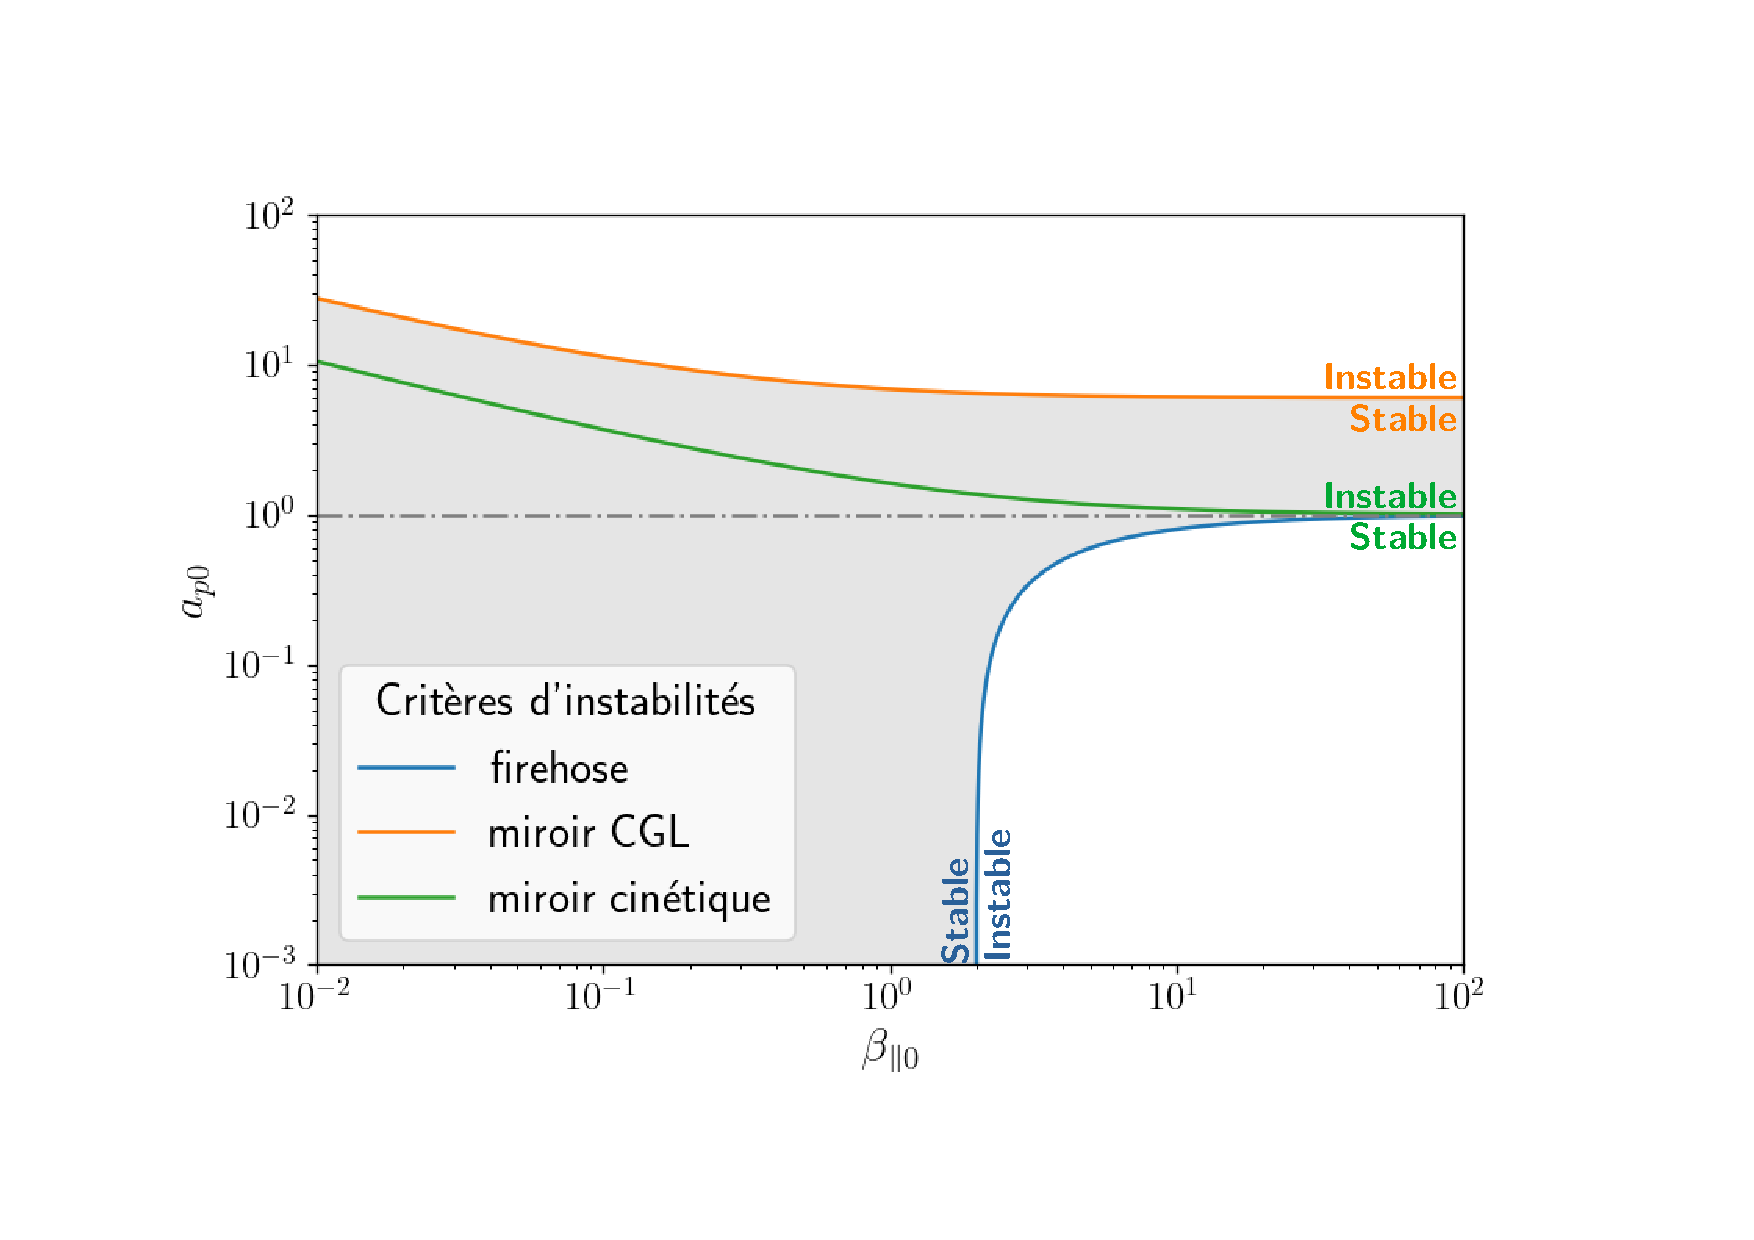
\includegraphics[width=0.7\linewidth,trim=3cm 2cm 4cm 3cm, clip=true]{./Part_2/images/crit_diag_CGL}
\caption{Zones de stabilité du modèle \ac{CGL} (zone grisée). Critères d'instabilité firehose (bleu), miroir (orange) et miroir cinétique (vert). Horizontale $a_p=1$ en gris.}
\label{fig:diag_cgl}
\end{figure}
L'expression du critère d'instabilité miroir est légèrement différente de celle provenant de la théorie linéaire cinétique à cause du facteur $1/6$ [\cite{galeev_mhd_1983,ferriere_mixed_2002}]. Ce facteur d'erreur translate la condition nécessaire pour qu'il y ait des instabilités miroir à $a_{p0}>6$ au lieu de $a_{p0}>1$ comme on peut le voir sur la \figref{fig:diag_cgl}. La condition nécessaire pour qu'il y ait apparition d'instabilité firehose est, quant à elle, $a_{p0}<1$ et en accord avec la théorie cinétique. Dans le vent solaire, ces critères d'instabilité semblent avoir un impact majeur puisque l'état du plasma semble maintenu, sur les diagrammes $a_p-\beta_{\parallel}$, dans une zone qu'ils semblent délimiter, comme l'a observé \cite{hellinger_solar_2006} dans les données relevées par la sonde \acs{WIND}. 

Dans le Chapitre \ref{ch-11}, nous avons rappelé l'importance des ondes d'Alfvén dans les théories de turbulence et, dans le Chapitre \ref{ch-12}, que le sujet de l'impact des ondes compressibles \ac{MHD} sur la cascade turbulente est toujours ouvert [\cite{brodiano_spatiotemporal_2021}]. Similairement, on peut se demander quel impact ont les instabilités sur la turbulence ? Et en particulier, quelle influence ont les instabilités des ondes d'Alfvén sur la turbulence Alfvénique ? 
\begin{figure}[!ht]
 \centering
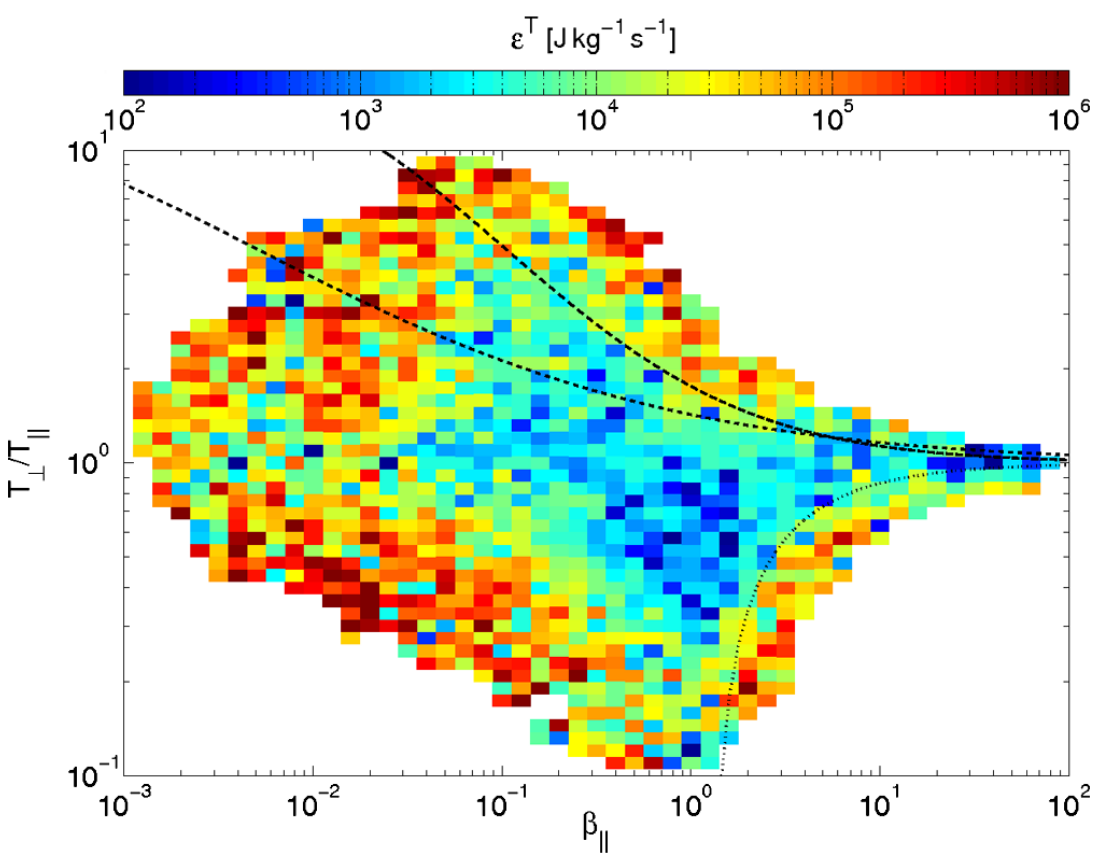
\includegraphics[width=0.7\linewidth,trim=0cm 0cm 0cm 0cm, clip=true]{./Part_2/images/osman_2013}
\caption{Distribution statistique en fonction de $a_p = \frac{p_{\perp}}{p_{\parallel}} =  \frac{T_{\perp}}{T_{\parallel}}$ et $\beta_{\parallel}$ d'échantillons relevés entre 1995 et 2011 dans le vent solaire par la sonde \acs{WIND} en orbite autour de la Terre. Pour chacun d'eux, le taux de cascade est calculé avec la loi exacte PP98 et indiqué par l'échelle chromatique. Les lignes indiquent les frontières associées aux instabilités cinétiques miroir (décroissante supérieure), cyclotron (décroissante inférieure) et firehose (croissante). Crédits : [\cite{osman_proton_2013}]. }
\label{fig:diag_osman}
\end{figure}
Si l'on regarde les résultats de l'étude de la température isotrope [\cite{liu_thermodynamic_2006}], des fluctuations magnétiques [\cite{bale_magnetic_2009}] et du taux de cascade incompressible [\cite{osman_proton_2013}] (voir \figref{fig:diag_osman}) dans les données relevées par \acs{WIND} et ceux du taux compressible isotherme observés par \cite{hadid_compressible_2018} dans les données des missions \acs{THEMIS} et \acs{CLUSTER} : sur les diagrammes $a_p-\beta_{\parallel}$, près des frontières des zones instables, la température des protons semble plus élevée, les fluctuations du champ magnétique et les taux de cascade plus importants. Mais la relation entre instabilités et turbulence reste à clarifier : est-ce que le plasma est plus chaud et turbulent parce que les instabilités jouent un rôle dans son chauffage ? Et est-ce que ce chauffage s'effectue via la cascade turbulente ? Est-ce lié à l'âge collisionnel du plasma comme le propose \cite{bale_magnetic_2009} ?

De multiples études se sont attaquées à ces questions à travers des études comparatives de spectres, du taux d'anisotropie de pression et des taux de croissance des instabilités cinétiques linéaires et quasi-linéaires (quelques études récentes : [\cite{qudsi_intermittency_2020,markovskii_effect_2022,opie_conditions_2022,bandyopadhyay_interplay_2022,navarro_effects_2023}]). 
De notre côté, nous l'attaquons analytiquement, à partir des échelles fluides et de la théorie des lois exactes, dans le but d'offrir un cadre fluide permettant d'étudier plus rigoureusement l'impact des anisotropies et instabilités de pression sur la cascade turbulente.

\section{Loi exacte générale pour pression tensorielle et \acs{CGL}}
\label{sec-213}

Pour obtenir une loi exacte pour le modèle \ac{CGL}, nous avons utilisé la méthode mise en place dans le Chapitre \ref{ch-13} : prendre en compte l'équation d'énergie interne \eqref{eq:model_cpg_u} et non la forme explicite des pressions parallèle et perpendiculaire \eqref{eq:model_cpg_biadiab}. Le modèle utilisé est donc :
\begin{eqnarray}
\label{eq:turb_cpg_r} \partial_t \rho &=& - \nabla \cdot \left(\rho \boldsymbol{v}\right) , \\
\label{eq:turb_cpg_v}\partial_t  \boldsymbol{v} &=&- \nabla \cdot \left(\boldsymbol{v}\boldsymbol{v}\right) + \boldsymbol{v} \nabla \cdot \boldsymbol{v}  + \frac{1}{\rho} \nabla \cdot \left(\rho \boldsymbol{v_A}\boldsymbol{v_A}\right) - \frac{1}{\rho}  \nabla \cdot \overline{\boldsymbol{P_*}}  + \boldsymbol{f_c} + \boldsymbol{d_c} ,\\
\label{eq:turb_cpg_b}\partial_t \boldsymbol{v_A} &=&   \nabla \cdot \left(\boldsymbol{v_A}\boldsymbol{v} - \boldsymbol{v}\boldsymbol{v_A}\right) -  \boldsymbol{v}  \nabla \cdot \boldsymbol{v_A} +  \frac{\boldsymbol{v_A}}{2}  \nabla \cdot \boldsymbol{v} + \boldsymbol{f_m} + \boldsymbol{d_m} ,\\
\label{eq:turb_cpg_u}    \partial_t u  &=& - \nabla \cdot \left(u \boldsymbol{v} \right) + u  \nabla \cdot \boldsymbol{v}  -  \frac{\overline{\boldsymbol{P}}}{\rho} : \nabla \boldsymbol{v} . 
\end{eqnarray}

De manière cohérente avec les choix effectués dans le Chapitre \ref{ch-13}, la fonction de corrélation d'énergie totale choisie est : $\mathcal{R} = \mathcal{R}_{c} + \mathcal{R}_{m} + \mathcal{R}_{u}$ avec $\mathcal{R}_{c} = \left<\frac{1}{4} \left(\rho'+\rho\right) \boldsymbol{v'} \cdot  \boldsymbol{v} \right>$, $\mathcal{R}_{m} = \left<\frac{1}{4} \left(\rho'+\rho\right) \boldsymbol{v'_A} \cdot  \boldsymbol{v_A} \right>$ et $\mathcal{R}_{u} = \frac{1}{2}\left< \rho' u + \rho u'\right> $. 

Et, en appliquant la  même méthode que celle utilisée pour obtenir \eqref{eq:turb_cpi_Rc}, \eqref{eq:turb_cpi_Rm} et \eqref{eq:turb_cpi_Ru}, on obtient l'évolution temporelle des fonctions de corrélation associées à chaque énergie : 
\begin{itemize}
    \item Énergie cinétique : $\mathcal{R}_{c} = \left<\left(\rho'+\rho\right)\boldsymbol{v'} \cdot \boldsymbol{v}\right>/4 $
\begin{eqnarray}
\label{eq:turb_cpg_Rc} 4\partial_t \mathcal{R}_{c} &=& \nabla_{\boldsymbol{\ell}} \cdot \left<\delta \left(\rho\boldsymbol{v}\right) \cdot \delta \boldsymbol{v} \delta \boldsymbol{v} -\left(\delta \left(\rho\boldsymbol{v_A}\right) \cdot \delta \boldsymbol{v} \delta \boldsymbol{v_A} + \delta \left(\rho\boldsymbol{v}\right) \cdot \delta \boldsymbol{v_A} \delta \boldsymbol{v_A} \right)\right>\nonumber \\
&+& \nabla_{\boldsymbol{\ell}} \cdot \left<\rho' \boldsymbol{v'_A}\cdot  \boldsymbol{v} \boldsymbol{v_A} -\rho \boldsymbol{v_A}\cdot  \boldsymbol{v'} \boldsymbol{v'_A}-\rho' \boldsymbol{v'} \cdot\boldsymbol{v_A}\boldsymbol{v'_A} +  \rho  \boldsymbol{v} \cdot\boldsymbol{v'_A}\boldsymbol{v_A}\right> \nonumber\\
& +&\left<\delta \boldsymbol{v}\cdot \left( \rho \boldsymbol{v}  \nabla' \cdot \boldsymbol{v'} -\rho' \boldsymbol{v'} \nabla \cdot \boldsymbol{v} \right)+2 \delta \boldsymbol{v_A}\cdot \left( \rho' \boldsymbol{v'} \nabla \cdot \boldsymbol{v_A} - \rho \boldsymbol{v} \right) \nabla' \cdot \boldsymbol{v'_A}\right> \nonumber\\
&+&  \nabla_{\boldsymbol{\ell}} \cdot \left< \rho' \frac{ \overline{\boldsymbol{P_*}}}{\rho} \cdot \boldsymbol{v'} -  \rho \frac{\overline{\boldsymbol{P'_*}}}{\rho'} \cdot \boldsymbol{v} + \overline{\boldsymbol{P_*}} \cdot \boldsymbol{v'} -  \overline{\boldsymbol{P'_*}} \cdot \boldsymbol{v} \right>\nonumber \\
&-& \left<\frac{\rho'}{\rho} \boldsymbol{v'} \cdot \overline{\boldsymbol{P_*}}  \cdot \frac{\nabla \rho}{\rho} + \frac{\rho}{\rho'} \boldsymbol{v} \cdot \overline{\boldsymbol{P'_*}}   \cdot \frac{\nabla' \rho'}{\rho'} \right>\nonumber\\
&+&  \left<\left(\rho' + \rho\right)\left(\boldsymbol{v} \cdot \boldsymbol{f'_c} + \boldsymbol{v'} \cdot \boldsymbol{f_c}\right) \right>+ \left<\left(\rho' + \rho\right)\left(\boldsymbol{v} \cdot \boldsymbol{d'_c} + \boldsymbol{v'} \cdot \boldsymbol{d_c}\right)\right> .
\end{eqnarray}
    \item Énergie magnétique : $\mathcal{R}_{m} = \left<\left(\rho'+\rho\right)\boldsymbol{v'_A} \cdot \boldsymbol{v_A}\right>/4 $
\begin{eqnarray}
\label{eq:turb_cpg_Rm} 4\partial_t \mathcal{R}_{m} &=& \nabla_{\boldsymbol{\ell}} \cdot \left<\delta \left(\rho\boldsymbol{v_A}\right) \cdot \delta \boldsymbol{v_A} \delta \boldsymbol{v} \right> \nonumber\\
&&-\nabla_{\boldsymbol{\ell}} \cdot \left< \rho' \boldsymbol{v'_A}\cdot  \boldsymbol{v} \boldsymbol{v_A} - \rho \boldsymbol{v_A}\cdot  \boldsymbol{v'} \boldsymbol{v'_A}-\rho' \boldsymbol{v'} \cdot\boldsymbol{v_A}\boldsymbol{v'_A} +  \rho  \boldsymbol{v} \cdot\boldsymbol{v'_A}\boldsymbol{v_A}\right> \nonumber\\
&&+ \left<\left(\rho \boldsymbol{v_A} \cdot \delta \boldsymbol{v_A} -\frac{1}{2} \left(\rho'+\rho\right) \boldsymbol{v'_A} \cdot \boldsymbol{v_A}\right)\nabla' \cdot \boldsymbol{v'}\right> \nonumber\\
&&-  \left<\left(\rho' \boldsymbol{v'_A} \cdot \delta \boldsymbol{v_A} + \frac{1}{2} \left(\rho'+\rho\right) \boldsymbol{v'_A} \cdot \boldsymbol{v_A}\right)\nabla \cdot \boldsymbol{v}\right>\nonumber\\
&& + \left<\left( \rho' \boldsymbol{v'_A} \cdot \boldsymbol{v} - \rho \boldsymbol{v} \cdot \boldsymbol{v'_A}  \right)\nabla \cdot \boldsymbol{v_A} \right> + \left<\left(\rho' \boldsymbol{v'} \cdot \boldsymbol{v_A} -  \rho \boldsymbol{v_A} \cdot \boldsymbol{v'} \right)\nabla' \cdot \boldsymbol{v'_A} \right>\nonumber\\
&&+  \left<\left(\rho' + \rho\right)\left(\boldsymbol{v_A} \cdot \boldsymbol{f'_m} + \boldsymbol{v'_A} \cdot \boldsymbol{f_m}\right) \right>+ \left<\left(\rho' + \rho\right)\left(\boldsymbol{v_A} \cdot \boldsymbol{d'_m} + \boldsymbol{v'_A} \cdot \boldsymbol{d_m}\right)\right> .\nonumber\\
\end{eqnarray}
    \item Énergie interne :  $\mathcal{R}_{u} = \left<\rho' u+\rho u'\right>/2 $
\begin{eqnarray}
\label{eq:turb_cpg_Ru} 2\partial_t \mathcal{R}_{u} &=&\nabla_{\boldsymbol{\ell}} \cdot \left<\delta \rho  \delta u \delta \boldsymbol{v} \right> + \left<  \rho \delta u \nabla' \cdot \boldsymbol{v'}- \rho' \delta u \nabla \cdot \boldsymbol{v}\right> \nonumber\\
&&-\left< \rho' \frac{\overline{\boldsymbol{P}}}{\rho} :  \nabla  \boldsymbol{v}  + \rho \frac{\overline{\boldsymbol{P'}}}{\rho'} : \nabla'  \boldsymbol{v'} \right> .
\end{eqnarray}
\end{itemize}
Le résultat pour l'énergie magnétique n'est pas influencé par le type de pression (tensoriel ou isotrope) contrairement à ceux des énergies cinétique et interne. La question qui s'est posée alors était : est-il possible d'améliorer la formulation des termes dépendants de la pression ? de faire apparaître l'influence de la pression dans les termes de type flux sous la forme d'une fonction de structure ?
En remarquant que $\overline{\boldsymbol{P}}$ ou $\overline{\boldsymbol{P_*}}$ est, dans tous les termes, accompagné de $\frac{1}{\rho}$ pris au même point, l'idée de travailler sur la fonction de structure $\left<\delta \rho \delta \frac{ \overline{\boldsymbol{P}}}{\rho} \cdot \delta \boldsymbol{v} \right>$ puis sur la fonction $\left<\delta \rho \delta \frac{ \overline{\boldsymbol{P_*}} }{\rho} \cdot\delta \boldsymbol{v} \right>$ a émergé. Développer cette dernière sous la divergence locale en utilisant l'hypothèse d'homogénéité statistique et l'indépendance des positions $\boldsymbol{x}$ et  $\boldsymbol{x'}$ donne : 
\begin{eqnarray*}
    \nabla_{\boldsymbol{\ell}} \cdot \left<\delta \rho \delta \frac{ \overline{\boldsymbol{P_*}} }{\rho}  \cdot\delta \boldsymbol{v} \right> &=& \nabla_{\boldsymbol{\ell}} \cdot \left< \left[\rho  \frac{ \overline{\boldsymbol{P'_*}} }{\rho'}   \cdot\boldsymbol{v}  -\rho'  \frac{ \overline{\boldsymbol{P_*}} }{\rho} \cdot \boldsymbol{v'}\right] +  \left[\overline{\boldsymbol{P_*}} \cdot \boldsymbol{v'} - \overline{\boldsymbol{P'_*}}    \cdot\boldsymbol{v} \right] \right> \\
    &&+\nabla_{\boldsymbol{\ell}} \cdot \left<\rho'  \frac{ \overline{\boldsymbol{P_*}} }{\rho} \cdot \boldsymbol{v} - \rho  \frac{ \overline{\boldsymbol{P'_*}} }{\rho'}  \cdot \boldsymbol{v'}  \right> .
\end{eqnarray*}
On va donc pouvoir remplacer $ \nabla_{\boldsymbol{\ell}} \cdot \left< \rho' \frac{ \overline{\boldsymbol{P_*}}}{\rho} \cdot \boldsymbol{v'} -  \rho \frac{\overline{\boldsymbol{P'_*}}}{\rho'} \cdot \boldsymbol{v} \right>$ ou $ \nabla_{\boldsymbol{\ell}} \cdot \left<  \overline{\boldsymbol{P_*}} \cdot \boldsymbol{v'} -  \overline{\boldsymbol{P'_*}} \cdot \boldsymbol{v} \right>$ dans \eqref{eq:turb_cpg_Rc}. En voyant que $ \nabla_{\boldsymbol{\ell}} \cdot \left<  \overline{\boldsymbol{P_*}} \cdot \boldsymbol{v'} -  \overline{\boldsymbol{P'_*}} \cdot \boldsymbol{v} \right>$ s'écrit aussi $\left<  \rho  \frac{ \overline{\boldsymbol{P_*}} }{\rho} : \nabla'\boldsymbol{v'} +   \rho'\frac{ \overline{\boldsymbol{P'_*}} }{\rho'} : \nabla \boldsymbol{v} \right>$ qui rappelle les termes dépendant de la pression de l'équation \eqref{eq:turb_cpg_Ru}, nous avons choisi la première possibilité. Ainsi : 
\begin{eqnarray*}
\nabla_{\boldsymbol{\ell}} &\cdot& \left< \rho' \frac{ \overline{\boldsymbol{P_*}}}{\rho} \cdot \boldsymbol{v'} -  \rho \frac{\overline{\boldsymbol{P'_*}}}{\rho'} \cdot \boldsymbol{v}  +  \overline{\boldsymbol{P_*}} \cdot \boldsymbol{v'} -  \overline{\boldsymbol{P'_*}} \cdot \boldsymbol{v} \right>\\
&=& -\nabla_{\boldsymbol{\ell}} \cdot \left<\delta \rho \delta \frac{ \overline{\boldsymbol{P_*}} }{\rho} \cdot \delta \boldsymbol{v} \right> +  \left<   \boldsymbol{v}\cdot\frac{ \overline{\boldsymbol{P_*}} }{\rho} \cdot  \nabla'\rho' + \boldsymbol{v'} \cdot \frac{ \overline{\boldsymbol{P'_*}} }{\rho'} \cdot \nabla \rho  \right> \\
&&+ \left< 2 \rho  \frac{ \overline{\boldsymbol{P}} }{\rho} : \nabla'\boldsymbol{v'} + 2  \rho'\frac{ \overline{\boldsymbol{P'}} }{\rho'} : \nabla \boldsymbol{v}  + \rho \boldsymbol{v_A}^2 \nabla' \cdot \boldsymbol{v'} +   \rho' \boldsymbol{v'_A}^2 \nabla \cdot \boldsymbol{v}\right> .
\end{eqnarray*}
La loi \acs{KHM} générale pour l'énergie totale avec $\mathcal{R} = \mathcal{R}_{c} + \mathcal{R}_{m} + \mathcal{R}_{u}$ devient alors :
\begin{equation}
\label{eq:turb_cpg_khm} \boxed{
\begin{array}{lcl}
{}_{[1]} \quad 4\partial_t \mathcal{R} &=& \nabla_{\boldsymbol{\ell}} \cdot \left<\left(\delta \left(\rho\boldsymbol{v}\right) \cdot \delta \boldsymbol{v}+ \delta \left(\rho\boldsymbol{v_A}\right) \cdot \delta \boldsymbol{v_A} \right) \delta \boldsymbol{v}  -\left(\delta \left(\rho\boldsymbol{v_A}\right) \cdot \delta \boldsymbol{v}  + \delta \left(\rho\boldsymbol{v}\right) \cdot \delta \boldsymbol{v_A}  \right) \delta \boldsymbol{v_A} \right>\\
{}_{[2]} && +\left< \left(\rho \boldsymbol{v} \cdot \delta \boldsymbol{v} +\frac{1}{2} \rho \boldsymbol{v_A} \cdot  \delta \boldsymbol{v_A} -\frac{1}{2} \delta \left(\rho \boldsymbol{v_A}\right) \cdot \boldsymbol{v_A} \right) \nabla' \cdot \boldsymbol{v'} \right>\\
{}_{[3]} && -\left< \left(\rho' \boldsymbol{v'} \cdot \delta \boldsymbol{v}  + \frac{1}{2} \rho' \boldsymbol{v'_A} \cdot \delta \boldsymbol{v_A}  - \frac{1}{2} \delta \left(\rho \boldsymbol{v_A}\right) \cdot \boldsymbol{v'_A}  \right)\nabla \cdot \boldsymbol{v}\right>\\
{}_{[4]} &&+ \left<\left(2 \rho' \boldsymbol{v'} \cdot \delta \boldsymbol{v_A}- \delta \left(\rho \boldsymbol{v}\right) \cdot \boldsymbol{v'_A} + \rho' \boldsymbol{v'_A} \cdot \delta \boldsymbol{v}  \right)\nabla \cdot \boldsymbol{v_A}\right>\\
{}_{[5]} &&- \left<\left(2\rho \boldsymbol{v} \cdot \delta \boldsymbol{v_A} - \delta \left(\rho \boldsymbol{v}\right) \cdot \boldsymbol{v_A} +  \rho \boldsymbol{v_A} \cdot \delta \boldsymbol{v} \right)\nabla' \cdot \boldsymbol{v'_A}\right> \\
{}_{[6]} &&+ \nabla_{\boldsymbol{\ell}} \cdot \left< 2\delta \rho  \delta u \delta \boldsymbol{v}\right> + 2\left<\rho \delta u \nabla' \cdot \boldsymbol{v'}- \rho' \delta u \nabla \cdot \boldsymbol{v}\right>\\
{}_{[7]} &&- \nabla_{\boldsymbol{\ell}} \cdot \left<\delta \rho \delta \frac{ \overline{\boldsymbol{P_*}} }{\rho} \cdot \delta \boldsymbol{v} \right> - 2\left<\rho \delta \frac{ \overline{\boldsymbol{P}} }{\rho}:\nabla' \boldsymbol{v'} -  \rho' \delta \frac{ \overline{\boldsymbol{P}} }{\rho} :\nabla  \boldsymbol{v} \right>\\
{}_{[8]} && +  \left< \boldsymbol{v} \cdot \left(  \frac{ \overline{\boldsymbol{P_*}} }{\rho} \delta \rho - \rho \delta \frac{ \overline{\boldsymbol{P_*}} }{\rho}  \right)\cdot  \frac{\nabla' \rho'}{\rho'} - \boldsymbol{v'} \cdot \left(  \frac{ \overline{\boldsymbol{P'_*}} }{\rho'} \delta \rho - \rho' \delta \frac{ \overline{\boldsymbol{P_*}} }{\rho}  \right)\cdot  \frac{\nabla \rho}{\rho}  \right>\\
{}_{[9]}&&+  \left<\left(\rho' + \rho\right)\left(\boldsymbol{v} \cdot \boldsymbol{f'_c} + \boldsymbol{v'} \cdot \boldsymbol{f_c} + \boldsymbol{v_A} \cdot \boldsymbol{f'_m} + \boldsymbol{v'_A} \cdot \boldsymbol{f_m}\right) \right>\\
{}_{[10]}&&+ \left<\left(\rho' + \rho\right)\left(\boldsymbol{v} \cdot \boldsymbol{d'_c} + \boldsymbol{v'} \cdot \boldsymbol{d_c}+\boldsymbol{v_A} \cdot \boldsymbol{d'_m} + \boldsymbol{v'_A} \cdot \boldsymbol{d_m}\right)\right> .
\end{array}}
\end{equation} 
Les lignes [7] et [8] contiennent les contributions des tenseurs de pression et de pression totale. 
La loi exacte générale de type \acs{K41} est alors : 
\begin{equation}
\label{eq:turb_cpg_elk} \boxed{
\begin{array}{lcl}
- 4\varepsilon &=& \nabla_{\boldsymbol{\ell}} \cdot \left<\left(\delta \left(\rho\boldsymbol{v}\right) \cdot \delta \boldsymbol{v}+ \delta \left(\rho\boldsymbol{v_A}\right) \cdot \delta \boldsymbol{v_A} \right) \delta \boldsymbol{v}  -\left(\delta \left(\rho\boldsymbol{v_A}\right) \cdot \delta \boldsymbol{v}  + \delta \left(\rho\boldsymbol{v}\right) \cdot \delta \boldsymbol{v_A}  \right) \delta \boldsymbol{v_A} \right>\\
&&+ \nabla_{\boldsymbol{\ell}} \cdot \left< 2\delta \rho  \delta u \delta \boldsymbol{v}-\delta \rho \delta \frac{ \overline{\boldsymbol{P_*}} }{\rho} \cdot \delta \boldsymbol{v} \right> \\
&& +\left< \left(\rho \boldsymbol{v} \cdot \delta \boldsymbol{v} +\frac{1}{2} \rho \boldsymbol{v_A} \cdot  \delta \boldsymbol{v_A} -\frac{1}{2} \delta \left(\rho \boldsymbol{v_A}\right) \cdot \boldsymbol{v_A} +2\rho \delta u\right) \nabla' \cdot \boldsymbol{v'} -2\rho \delta \frac{ \overline{\boldsymbol{P}} }{\rho}:\nabla' \boldsymbol{v'}\right>\\
 && -\left< \left(\rho' \boldsymbol{v'} \cdot \delta \boldsymbol{v}  + \frac{1}{2} \rho' \boldsymbol{v'_A} \cdot \delta \boldsymbol{v_A}  - \frac{1}{2} \delta \left(\rho \boldsymbol{v_A}\right) \cdot \boldsymbol{v'_A}  +2\rho' \delta u\right)\nabla \cdot \boldsymbol{v} - 2\rho' \delta \frac{ \overline{\boldsymbol{P}} }{\rho} :\nabla  \boldsymbol{v}\right>\\
&&+ \left<\left(2 \rho' \boldsymbol{v'} \cdot \delta \boldsymbol{v_A}- \delta \left(\rho \boldsymbol{v}\right) \cdot \boldsymbol{v'_A} + \rho' \boldsymbol{v'_A} \cdot \delta \boldsymbol{v}  \right)\nabla \cdot \boldsymbol{v_A}\right>\\
 &&- \left<\left(2\rho \boldsymbol{v} \cdot \delta \boldsymbol{v_A} - \delta \left(\rho \boldsymbol{v}\right) \cdot \boldsymbol{v_A} +  \rho \boldsymbol{v_A} \cdot \delta \boldsymbol{v} \right)\nabla' \cdot \boldsymbol{v'_A}\right> \\
&& +  \left< \boldsymbol{v} \cdot \left(  \frac{ \overline{\boldsymbol{P_*}} }{\rho} \delta \rho - \rho \delta \frac{ \overline{\boldsymbol{P_*}} }{\rho}  \right)\cdot  \frac{\nabla' \rho'}{\rho'} - \boldsymbol{v'} \cdot \left(  \frac{ \overline{\boldsymbol{P'_*}} }{\rho'} \delta \rho - \rho' \delta \frac{ \overline{\boldsymbol{P_*}} }{\rho}  \right)\cdot  \frac{\nabla \rho}{\rho}  \right>.
\end{array}}
\end{equation}
Cette loi est valable quelle que soit la forme du tenseur de pression ou de l'énergie interne tant que la zone inertielle est supposée isentrope. Si l'on considère la pression sous forme isotrope $\overline{\boldsymbol{P}} = p \overline{\boldsymbol{I}}$, on trouve la loi \eqref{eq:turb_elg_f2} analysée dans la section \ref{sec-132}. On va noter ce résultat $\varepsilon_{iso}$. On peut alors isoler, dans le taux de cascade, la contribution de la composante anisotrope du tenseur de pression $\overline{\boldsymbol{\Pi}}$ : 
\begin{equation}
\label{eq:turb_cpgyr_an} \boxed{
\begin{array}{lcl}
- 4\left(\varepsilon - \varepsilon_{iso}\right) &=& - \nabla_{\boldsymbol{\ell}} \cdot \left< \delta \rho \delta \left(\frac{\overline{\boldsymbol{\Pi}}}{\rho}\right) \cdot \delta \boldsymbol{v} \right>  -\left< 2\rho \delta \left(\frac{\overline{\boldsymbol{\Pi}}}{\rho}\right):\nabla' \boldsymbol{v'} -  2\rho' \delta \left(\frac{\overline{\boldsymbol{\Pi}}}{\rho}\right) :\nabla  \boldsymbol{v}\right>\\
&& +  \left< \boldsymbol{v} \cdot \left(  \left(\frac{\overline{\boldsymbol{\Pi}}}{\rho}\right) \delta \rho - \rho \delta \left(\frac{\overline{\boldsymbol{\Pi}}}{\rho}\right)  \right)\cdot  \frac{\nabla' \rho'}{\rho'}-\boldsymbol{v'} \cdot \left(  \left(\frac{\overline{\boldsymbol{\Pi'}}}{\rho'}\right) \delta \rho - \rho' \delta \left(\frac{\overline{\boldsymbol{\Pi}}}{\rho}\right)  \right)\cdot  \frac{\nabla \rho}{\rho}  \right>.
\end{array}}
\end{equation}
Nous quantifierons et analyserons cette contribution grâce à des simulations dans la Partie \ref{part_3}. 

Dans le cas d'un tenseur de pression gyrotrope, on peut faire apparaître $p_{\parallel}$ et $p_{\perp}$ : 
\begin{eqnarray}
\label{eq:turb_cpgyr_elk} 
- 4\varepsilon &=& \nabla_{\boldsymbol{\ell}} \cdot \left<\left(\delta \left(\rho\boldsymbol{v}\right) \cdot \delta \boldsymbol{v}+ \delta \left(\rho\boldsymbol{v_A}\right) \cdot \delta \boldsymbol{v_A} \right)\delta \boldsymbol{v}  -\left(\delta \left(\rho\boldsymbol{v_A}\right) \cdot \delta \boldsymbol{v}  + \delta \left(\rho\boldsymbol{v}\right) \cdot \delta \boldsymbol{v_A}  \right) \delta \boldsymbol{v_A} \right>\nonumber\\
&+& \nabla_{\boldsymbol{\ell}} \cdot \left< \delta \rho  \delta \left(\frac{p_{\perp} + p_{\parallel}+p_m}{\rho}\right) \delta \boldsymbol{v}+\delta \rho \delta \left(\frac{p_{\perp} - p_{\parallel}}{\rho}\boldsymbol{b}\boldsymbol{b}\right) \cdot \delta \boldsymbol{v} \right>\nonumber \\
& +&\left< \left(\rho \boldsymbol{v} \cdot \delta \boldsymbol{v} +\frac{1}{2} \rho \boldsymbol{v_A} \cdot  \delta \boldsymbol{v_A} -\frac{1}{2} \delta \left(\rho \boldsymbol{v_A}\right) \cdot \boldsymbol{v_A} +\rho \delta \left(\frac{p_{\parallel}}{\rho}\right)\right) \nabla' \cdot \boldsymbol{v'} \right>\nonumber\\
 & -&\left< \left(\rho' \boldsymbol{v'} \cdot \delta \boldsymbol{v}  + \frac{1}{2} \rho' \boldsymbol{v'_A} \cdot \delta \boldsymbol{v_A}  - \frac{1}{2} \delta \left(\rho \boldsymbol{v_A}\right) \cdot \boldsymbol{v'_A}  +\rho' \delta \left(\frac{p_{\parallel}}{\rho}\right)\right)\nabla \cdot \boldsymbol{v} \right>\nonumber\\
 &+&2\left<\rho \delta \left(\frac{p_{\perp} - p_{\parallel}}{\rho}\boldsymbol{b}\boldsymbol{b}\right):\nabla' \boldsymbol{v'} - \rho' \delta \left(\frac{p_{\perp} - p_{\parallel}}{\rho}\boldsymbol{b}\boldsymbol{b}\right) :\nabla  \boldsymbol{v}\right>\nonumber\\
&+& \left<\left(2 \rho' \boldsymbol{v'} \cdot \delta \boldsymbol{v_A}- \delta \left(\rho \boldsymbol{v}\right) \cdot \boldsymbol{v'_A} + \rho' \boldsymbol{v'_A} \cdot \delta \boldsymbol{v}  \right)\nabla \cdot \boldsymbol{v_A}\right>\nonumber\\
 &-& \left<\left(2\rho \boldsymbol{v} \cdot \delta \boldsymbol{v_A} - \delta \left(\rho \boldsymbol{v}\right) \cdot \boldsymbol{v_A} +  \rho \boldsymbol{v_A} \cdot \delta \boldsymbol{v} \right)\nabla' \cdot \boldsymbol{v'_A}\right> \nonumber\\
  % & +&  \left< \delta \rho  \left(  \frac{p_{\perp}+p_m }{\rho} \boldsymbol{v}\cdot  \frac{\nabla' \rho'}{\rho'} - \frac{ p'_{\perp}+p'_m }{\rho'} \boldsymbol{v'} \cdot  \frac{\nabla \rho}{\rho}\right) 
  % - \delta \left(\frac{ p_{\perp}+p_m }{\rho}\right) \left(\rho \boldsymbol{v} \cdot  \frac{\nabla' \rho'}{\rho'} -  \rho' \boldsymbol{v'}\cdot  \frac{\nabla \rho}{\rho}\right)  \right>\nonumber \\
  % &+& \left<  \delta \rho\left( \frac{ p_{\parallel}-p_{\perp}}{\rho} \boldsymbol{v} \cdot\boldsymbol{b}\boldsymbol{b}   \cdot  \frac{\nabla' \rho'}{\rho'} - \frac{ p'_{\parallel}-p'_{\perp}}{\rho'}\boldsymbol{v'} \cdot\boldsymbol{b'}\boldsymbol{b'}  \cdot  \frac{\nabla \rho}{\rho}\right)
  % -  \delta \left(\frac{ p_{\parallel}-p_{\perp}}{\rho}\boldsymbol{b}\boldsymbol{b} \right) : \left( \rho  \boldsymbol{v}  \frac{\nabla' \rho'}{\rho'} - \rho' \boldsymbol{v'}   \frac{\nabla \rho}{\rho} \right)\right>\nonumber \\
  & +&  \left<  \left(  \frac{p_{\perp}+p_m }{\rho} \boldsymbol{v}\delta \rho - \rho \boldsymbol{v}\delta \left(\frac{ p_{\perp}+p_m }{\rho}\right) \right)\cdot  \frac{\nabla' \rho'}{\rho'} \right>\nonumber \\
  &+&  \left<  \left(    \frac{ p_{\parallel}-p_{\perp}}{\rho} \boldsymbol{v} \cdot\boldsymbol{b}\boldsymbol{b} \delta \rho -\rho  \boldsymbol{v} \cdot \delta \left(\frac{ p_{\parallel}-p_{\perp}}{\rho}\boldsymbol{b}\boldsymbol{b} \right)  \right)\cdot  \frac{\nabla' \rho'}{\rho'} \right>\nonumber \\
 &-& \left< \left(  \frac{ p'_{\perp}+p'_m }{\rho'} \boldsymbol{v'}\delta \rho - \rho' \boldsymbol{v'}\delta \left(\frac{ p_{\perp}+p_m }{\rho}\right) \right) \cdot  \frac{\nabla \rho}{\rho} \right>\nonumber \\
 &-&   \left< \left(  \frac{ p'_{\parallel}-p'_{\perp}}{\rho'}\boldsymbol{v'} \cdot\boldsymbol{b'}\boldsymbol{b'}  \delta \rho - \rho' \boldsymbol{v'} \cdot\delta \left(\frac{ p_{\parallel}-p_{\perp}}{\rho}\boldsymbol{b}\boldsymbol{b} \right)\right) \cdot  \frac{\nabla \rho}{\rho} \right> .\nonumber\\
\end{eqnarray}
Cette loi est valable pour le modèle \ac{CGL}. Si besoin est, on peut y expliciter $p_{\parallel}$ et $p_{\perp}$ en fonction de $\rho$, $\boldsymbol{v_A}$ grâce à \eqref{eq:model_cpg_biadiab}. 

On peut aussi faire apparaître $a_p$ et $\beta_{\parallel}$ dans \eqref{eq:turb_cpgyr_elk} pour identifier les termes potentiellement impactés par les instabilités. Ainsi, on obtient :  
\begin{equation}
\label{eq:turb_cpinst_elk} \boxed{
\begin{array}{lcl}
- 4\varepsilon &=& \nabla_{\boldsymbol{\ell}} \cdot \left<\left(\delta \left(\rho\boldsymbol{v}\right) \cdot \delta \boldsymbol{v}+ \delta \left(\rho\boldsymbol{v_A}\right) \cdot \delta \boldsymbol{v_A} \right) \delta \boldsymbol{v}  -\left(\delta \left(\rho\boldsymbol{v_A}\right) \cdot \delta \boldsymbol{v}  + \delta \left(\rho\boldsymbol{v}\right) \cdot \delta \boldsymbol{v_A}  \right) \delta \boldsymbol{v_A} \right>\\
&&+ \frac{1}{2}\nabla_{\boldsymbol{\ell}} \cdot \left< \delta \rho  \delta \left(\boldsymbol{v_A}^2 \left(\beta_{\parallel}\left(a_p+1\right)+1\right)\right) \delta \boldsymbol{v}+\delta \rho \delta \left(\beta_{\parallel}\left(a_p-1\right) \boldsymbol{v_A} \boldsymbol{v_A}\right) \cdot \delta \boldsymbol{v} \right> \\
&& +\left< \left(\rho \boldsymbol{v} \cdot \delta \boldsymbol{v} +\frac{1}{2} \rho \boldsymbol{v_A} \cdot  \delta \boldsymbol{v_A} -\frac{1}{2} \delta \left(\rho \boldsymbol{v_A}\right) \cdot \boldsymbol{v_A} + \frac{1}{2}\rho \delta \left(\boldsymbol{v_A}^2 \beta_{\parallel}\right)\right) \nabla' \cdot \boldsymbol{v'} \right>\\
 && -\left< \left(\rho' \boldsymbol{v'} \cdot \delta \boldsymbol{v}  + \frac{1}{2} \rho' \boldsymbol{v'_A} \cdot \delta \boldsymbol{v_A}  - \frac{1}{2} \delta \left(\rho \boldsymbol{v_A}\right) \cdot \boldsymbol{v'_A}  + \frac{1}{2} \rho' \delta \left(\boldsymbol{v_A}^2 \beta_{\parallel}\right)\right)\nabla \cdot \boldsymbol{v} \right>\\
 &&+\left<\rho \delta \left(\beta_{\parallel}\left(a_p-1\right) \boldsymbol{v_A} \boldsymbol{v_A}\right):\nabla' \boldsymbol{v'} - \rho' \delta \left(\beta_{\parallel}\left(a_p-1\right) \boldsymbol{v_A} \boldsymbol{v_A}\right) :\nabla  \boldsymbol{v}\right>\\
&&+ \left<\left(2 \rho' \boldsymbol{v'} \cdot \delta \boldsymbol{v_A}- \delta \left(\rho \boldsymbol{v}\right) \cdot \boldsymbol{v'_A} + \rho' \boldsymbol{v'_A} \cdot \delta \boldsymbol{v}  \right)\nabla \cdot \boldsymbol{v_A}\right>\\
 &&- \left<\left(2\rho \boldsymbol{v} \cdot \delta \boldsymbol{v_A} - \delta \left(\rho \boldsymbol{v}\right) \cdot \boldsymbol{v_A} +  \rho \boldsymbol{v_A} \cdot \delta \boldsymbol{v} \right)\nabla' \cdot \boldsymbol{v'_A}\right> \\
&& + \frac{1}{2} \left<  \left(  \boldsymbol{v_A}^2 \left(\beta_{\parallel}a_p+1\right) \delta \rho - \rho \delta \left(\boldsymbol{v_A}^2 \left(\beta_{\parallel}a_p+1\right)\right)  \right)\boldsymbol{v}\cdot  \frac{\nabla' \rho'}{\rho'} \right>\\
&&- \frac{1}{2} \left<\left(  \boldsymbol{v'_A}^2 \left(\beta'_{\parallel}a'_p+1\right) \delta \rho - \rho' \delta \left(\boldsymbol{v_A}^2 \left(\beta_{\parallel}a_p+1\right)\right)  \right) \boldsymbol{v'}\cdot  \frac{\nabla \rho}{\rho}  \right> \\
&& + \frac{1}{2} \left< \boldsymbol{v} \cdot \left(  \beta_{\parallel}\left(a_p-1\right) \boldsymbol{v_A} \boldsymbol{v_A} \delta \rho - \rho \delta \left(\beta_{\parallel}\left(a_p-1\right) \boldsymbol{v_A} \boldsymbol{v_A}\right)  \right)\cdot  \frac{\nabla' \rho'}{\rho'} \right>\\
&&-\frac{1}{2}\left< \boldsymbol{v'} \cdot \left( \beta'_{\parallel}\left(a'_p-1\right) \boldsymbol{v'_A} \boldsymbol{v'_A}  \delta \rho - \rho' \delta \left(\beta_{\parallel}\left(a_p-1\right) \boldsymbol{v_A} \boldsymbol{v_A} \right)\right) \cdot  \frac{\nabla \rho}{\rho} \right>.
\end{array}}
\end{equation}
Les critères d'instabilité linéaires n'y sont pas explicites mais on voit que certains termes dépendent de $a_p-1$, en particulier un terme de type flux. Par conséquent, le signe de ces termes va dépendre du régime de pression dans le système, si $p_{\parallel}$ ou $p_{\perp}$ domine, et est ainsi lié au type d'instabilité pouvant s'y développer. Comme ces termes dépendent de quantités incrémentales, il est néanmoins difficile de conclure sur leur apport au taux de cascade total sans regarder dans des simulations. Ce sera l'un des objectifs de la Partie \ref{part_3}. On remarque que ces termes sont présents dans la contribution anisotrope \eqref{eq:turb_cpgyr_an} au taux de cascade.

\newpage
\section{Synthèse de l'étude analytique de turbulence compressible avec pression tensorielle et modèle \ac{CGL}}
\label{synt-21}

\fcolorbox{blue}{white}{\begin{minipage}[c]{\linewidth}
\paragraph{Fermeture \ac{CGL} : } $\nabla \cdot \overline{\overline{\boldsymbol{q}}}=0$ et $\overline{\boldsymbol{P}}  = p \overline{\boldsymbol{I}} + \overline{\boldsymbol{\Pi}}=  \frac{2 p_{\perp} + p_{\parallel}}{3}  \overline{\boldsymbol{I}} + \left(p_{\parallel} - p_{\perp}\right)\left(\boldsymbol{b}\boldsymbol{b} - \frac{1}{3} \overline{\boldsymbol{I}} \right)$ avec $\boldsymbol{b} = \frac{\boldsymbol{v_A}}{|\boldsymbol{v_A}|}$. Energie interne définie telle que $\rho u = \frac{3}{2}p$.
\begin{eqnarray}
\label{eq:synth_turbg_ppar}     \partial_t p_{\parallel} + \nabla \cdot \left(p_{\parallel} \boldsymbol{v} \right) + 2 p_{\parallel} \boldsymbol{b}\boldsymbol{b} : \nabla \boldsymbol{v}   &=& 0 ,\\
\label{eq:synth_turbg_pperp}     \partial_t p_{\perp} + \nabla \cdot \left(p_{\perp} \boldsymbol{v} \right) + p_{\perp} \nabla \cdot \boldsymbol{v}- p_{\perp} \boldsymbol{b}\boldsymbol{b} : \nabla \boldsymbol{v}   &=& 0 .
\end{eqnarray}

\paragraph{Linéarisation du modèle \ac{CGL} : }
\begin{itemize}
    \item Relation de dispersion : \eqref{eq:lin_cpg_disp}
    \item Mode d'Alfvén incompressible $\Rightarrow$ instabilité firehose,
    \item Mode magnétosonore rapide : stable,
    \item Mode magnétosonore lent $\Rightarrow$ instabilité firehose parallèle et miroir
    \item instabilité firehose si $1-\frac{\beta_{\parallel 0}}{2} \left(1-a_{p0}\right)<0$
    \item instabilité miroir si $1+\beta_{\parallel 0}a_{p0}\left(1-\frac{1}{6}a_{p0}\right)<0$
\end{itemize}
\end{minipage}}

\fcolorbox{red}{white}{\begin{minipage}[c]{\linewidth}
\paragraph{Equations utilisées pour calculer la loi exacte générale avec tenseur de pression (zone inertielle isentrope) : }
\begin{eqnarray}
\label{eq:synth_turbg_r} \partial_t \rho &=& - \nabla \cdot \left(\rho \boldsymbol{v}\right),  \\
\label{eq:synth_turbg_v}\partial_t  \boldsymbol{v} &=&- \nabla \cdot \left(\boldsymbol{v}\boldsymbol{v}\right) + \boldsymbol{v} \nabla \cdot \boldsymbol{v}  + \frac{1}{\rho} \nabla \cdot \left(\rho \boldsymbol{v_A}\boldsymbol{v_A}\right) - \frac{1}{\rho}  \nabla \cdot \overline{\boldsymbol{P_*}}  + \left(\boldsymbol{f_c} + \boldsymbol{d_c}\right) ,\\
\label{eq:synth_turbg_b}\partial_t \boldsymbol{v_A} &=&   \nabla \cdot \left(\boldsymbol{v_A}\boldsymbol{v} - \boldsymbol{v}\boldsymbol{v_A}\right) -  \boldsymbol{v}  \nabla \cdot \boldsymbol{v_A} +  \frac{\boldsymbol{v_A}}{2}  \nabla \cdot \boldsymbol{v} + \left(\boldsymbol{f_m} + \boldsymbol{d_m}\right), \\
\label{eq:synth_turbg_u}    \partial_t u  &=& - \nabla \cdot \left(u \boldsymbol{v} \right) + u  \nabla \cdot \boldsymbol{v}  -  \frac{\overline{\boldsymbol{P}}}{\rho} : \nabla \boldsymbol{v}  .
\end{eqnarray}

\paragraph{Fonctions de corrélation d'énergie totale considérée :\\}  $\mathcal{R} = \frac{1}{2} \left<\frac{1}{2} \left(\rho'+\rho\right) \boldsymbol{v'} \cdot  \boldsymbol{v} + \frac{1}{2} \left(\rho'+\rho\right) \boldsymbol{v'_A} \cdot  \boldsymbol{v_A} +  \rho' u + \rho u' \right>$. \\

\paragraph{Lois exactes générales dérivées dans ce chapitre (formulation f2) :} 
\begin{itemize}
    \item \acs{KHM} générale $\forall \overline{\boldsymbol{P}}$ :  \eqref{eq:turb_cpg_khm},
    \item \acs{K41} générale $\forall \overline{\boldsymbol{P}}$ :  \eqref{eq:turb_cpg_elk},
    \item contribution de l'anisotropie de pression :  \eqref{eq:turb_cpgyr_an}.
\end{itemize}
\paragraph{Lois exactes \acs{K41} gyrotrope/\ac{CGL} répondant à l'objectif initial (formulation f2) :} 
\begin{itemize}
    \item fonction de $p_{\parallel}$ et $p_{\perp}$ : \eqref{eq:turb_cpgyr_elk},
    \item fonction de $a_p = \frac{p_{\perp}}{p_{\parallel}}$ et $\beta_{\parallel} = \frac{p_{\parallel}}{p_m}$ : \eqref{eq:turb_cpinst_elk}.
\end{itemize}

Les résultats dérivés ici sont publiés dans [\cite{simon_exact_2022}]. 
\end{minipage}}
